
% Default to the notebook output style

    


% Inherit from the specified cell style.




    
\documentclass[10pt]{article}

    
    
    \usepackage[T1]{fontenc}
    % Nicer default font (+ math font) than Computer Modern for most use cases
    \usepackage{mathpazo}

    % Basic figure setup, for now with no caption control since it's done
    % automatically by Pandoc (which extracts ![](path) syntax from Markdown).
    \usepackage{graphicx}
    % We will generate all images so they have a width \maxwidth. This means
    % that they will get their normal width if they fit onto the page, but
    % are scaled down if they would overflow the margins.
    \makeatletter
    \def\maxwidth{\ifdim\Gin@nat@width>\linewidth\linewidth
    \else\Gin@nat@width\fi}
    \makeatother
    \let\Oldincludegraphics\includegraphics
    % Set max figure width to be 80% of text width, for now hardcoded.
    \renewcommand{\includegraphics}[1]{\Oldincludegraphics[width=.8\maxwidth]{#1}}
    % Ensure that by default, figures have no caption (until we provide a
    % proper Figure object with a Caption API and a way to capture that
    % in the conversion process - todo).
    \usepackage{caption}
    \DeclareCaptionLabelFormat{nolabel}{}
    \captionsetup{labelformat=nolabel}

    \usepackage{adjustbox} % Used to constrain images to a maximum size 
    \usepackage{xcolor} % Allow colors to be defined
    \usepackage{enumerate} % Needed for markdown enumerations to work
    \usepackage{geometry} % Used to adjust the document margins
    \usepackage{amsmath} % Equations
    \usepackage{amssymb} % Equations
    \usepackage{textcomp} % defines textquotesingle
    % Hack from http://tex.stackexchange.com/a/47451/13684:
    \AtBeginDocument{%
        \def\PYZsq{\textquotesingle}% Upright quotes in Pygmentized code
    }
    \usepackage{upquote} % Upright quotes for verbatim code
    \usepackage{eurosym} % defines \euro
    \usepackage[mathletters]{ucs} % Extended unicode (utf-8) support
    \usepackage[utf8x]{inputenc} % Allow utf-8 characters in the tex document
    \usepackage{fancyvrb} % verbatim replacement that allows latex
    \usepackage{grffile} % extends the file name processing of package graphics 
                         % to support a larger range 
    % The hyperref package gives us a pdf with properly built
    % internal navigation ('pdf bookmarks' for the table of contents,
    % internal cross-reference links, web links for URLs, etc.)
    \usepackage{hyperref}
    \usepackage{longtable} % longtable support required by pandoc >1.10
    \usepackage{booktabs}  % table support for pandoc > 1.12.2
    \usepackage[inline]{enumitem} % IRkernel/repr support (it uses the enumerate* environment)
    \usepackage[normalem]{ulem} % ulem is needed to support strikethroughs (\sout)
                                % normalem makes italics be italics, not underlines
    

    
    
    % Colors for the hyperref package
    \definecolor{urlcolor}{rgb}{0,.145,.698}
    \definecolor{linkcolor}{rgb}{.71,0.21,0.01}
    \definecolor{citecolor}{rgb}{.12,.54,.11}

    % ANSI colors
    \definecolor{ansi-black}{HTML}{3E424D}
    \definecolor{ansi-black-intense}{HTML}{282C36}
    \definecolor{ansi-red}{HTML}{E75C58}
    \definecolor{ansi-red-intense}{HTML}{B22B31}
    \definecolor{ansi-green}{HTML}{00A250}
    \definecolor{ansi-green-intense}{HTML}{007427}
    \definecolor{ansi-yellow}{HTML}{DDB62B}
    \definecolor{ansi-yellow-intense}{HTML}{B27D12}
    \definecolor{ansi-blue}{HTML}{208FFB}
    \definecolor{ansi-blue-intense}{HTML}{0065CA}
    \definecolor{ansi-magenta}{HTML}{D160C4}
    \definecolor{ansi-magenta-intense}{HTML}{A03196}
    \definecolor{ansi-cyan}{HTML}{60C6C8}
    \definecolor{ansi-cyan-intense}{HTML}{258F8F}
    \definecolor{ansi-white}{HTML}{C5C1B4}
    \definecolor{ansi-white-intense}{HTML}{A1A6B2}

    % commands and environments needed by pandoc snippets
    % extracted from the output of `pandoc -s`
    \providecommand{\tightlist}{%
      \setlength{\itemsep}{0pt}\setlength{\parskip}{0pt}}
    \DefineVerbatimEnvironment{Highlighting}{Verbatim}{commandchars=\\\{\}}
    % Add ',fontsize=\small' for more characters per line
    \newenvironment{Shaded}{}{}
    \newcommand{\KeywordTok}[1]{\textcolor[rgb]{0.00,0.44,0.13}{\textbf{{#1}}}}
    \newcommand{\DataTypeTok}[1]{\textcolor[rgb]{0.56,0.13,0.00}{{#1}}}
    \newcommand{\DecValTok}[1]{\textcolor[rgb]{0.25,0.63,0.44}{{#1}}}
    \newcommand{\BaseNTok}[1]{\textcolor[rgb]{0.25,0.63,0.44}{{#1}}}
    \newcommand{\FloatTok}[1]{\textcolor[rgb]{0.25,0.63,0.44}{{#1}}}
    \newcommand{\CharTok}[1]{\textcolor[rgb]{0.25,0.44,0.63}{{#1}}}
    \newcommand{\StringTok}[1]{\textcolor[rgb]{0.25,0.44,0.63}{{#1}}}
    \newcommand{\CommentTok}[1]{\textcolor[rgb]{0.38,0.63,0.69}{\textit{{#1}}}}
    \newcommand{\OtherTok}[1]{\textcolor[rgb]{0.00,0.44,0.13}{{#1}}}
    \newcommand{\AlertTok}[1]{\textcolor[rgb]{1.00,0.00,0.00}{\textbf{{#1}}}}
    \newcommand{\FunctionTok}[1]{\textcolor[rgb]{0.02,0.16,0.49}{{#1}}}
    \newcommand{\RegionMarkerTok}[1]{{#1}}
    \newcommand{\ErrorTok}[1]{\textcolor[rgb]{1.00,0.00,0.00}{\textbf{{#1}}}}
    \newcommand{\NormalTok}[1]{{#1}}
    
    % Additional commands for more recent versions of Pandoc
    \newcommand{\ConstantTok}[1]{\textcolor[rgb]{0.53,0.00,0.00}{{#1}}}
    \newcommand{\SpecialCharTok}[1]{\textcolor[rgb]{0.25,0.44,0.63}{{#1}}}
    \newcommand{\VerbatimStringTok}[1]{\textcolor[rgb]{0.25,0.44,0.63}{{#1}}}
    \newcommand{\SpecialStringTok}[1]{\textcolor[rgb]{0.73,0.40,0.53}{{#1}}}
    \newcommand{\ImportTok}[1]{{#1}}
    \newcommand{\DocumentationTok}[1]{\textcolor[rgb]{0.73,0.13,0.13}{\textit{{#1}}}}
    \newcommand{\AnnotationTok}[1]{\textcolor[rgb]{0.38,0.63,0.69}{\textbf{\textit{{#1}}}}}
    \newcommand{\CommentVarTok}[1]{\textcolor[rgb]{0.38,0.63,0.69}{\textbf{\textit{{#1}}}}}
    \newcommand{\VariableTok}[1]{\textcolor[rgb]{0.10,0.09,0.49}{{#1}}}
    \newcommand{\ControlFlowTok}[1]{\textcolor[rgb]{0.00,0.44,0.13}{\textbf{{#1}}}}
    \newcommand{\OperatorTok}[1]{\textcolor[rgb]{0.40,0.40,0.40}{{#1}}}
    \newcommand{\BuiltInTok}[1]{{#1}}
    \newcommand{\ExtensionTok}[1]{{#1}}
    \newcommand{\PreprocessorTok}[1]{\textcolor[rgb]{0.74,0.48,0.00}{{#1}}}
    \newcommand{\AttributeTok}[1]{\textcolor[rgb]{0.49,0.56,0.16}{{#1}}}
    \newcommand{\InformationTok}[1]{\textcolor[rgb]{0.38,0.63,0.69}{\textbf{\textit{{#1}}}}}
    \newcommand{\WarningTok}[1]{\textcolor[rgb]{0.38,0.63,0.69}{\textbf{\textit{{#1}}}}}
    
    
    % Define a nice break command that doesn't care if a line doesn't already
    % exist.
    \def\br{\hspace*{\fill} \\* }
    % Math Jax compatability definitions
    \def\gt{>}
    \def\lt{<}
    % Document parameters
    \title{sheet2}
    
    
    

    % Pygments definitions
    
\makeatletter
\def\PY@reset{\let\PY@it=\relax \let\PY@bf=\relax%
    \let\PY@ul=\relax \let\PY@tc=\relax%
    \let\PY@bc=\relax \let\PY@ff=\relax}
\def\PY@tok#1{\csname PY@tok@#1\endcsname}
\def\PY@toks#1+{\ifx\relax#1\empty\else%
    \PY@tok{#1}\expandafter\PY@toks\fi}
\def\PY@do#1{\PY@bc{\PY@tc{\PY@ul{%
    \PY@it{\PY@bf{\PY@ff{#1}}}}}}}
\def\PY#1#2{\PY@reset\PY@toks#1+\relax+\PY@do{#2}}

\expandafter\def\csname PY@tok@w\endcsname{\def\PY@tc##1{\textcolor[rgb]{0.73,0.73,0.73}{##1}}}
\expandafter\def\csname PY@tok@c\endcsname{\let\PY@it=\textit\def\PY@tc##1{\textcolor[rgb]{0.25,0.50,0.50}{##1}}}
\expandafter\def\csname PY@tok@cp\endcsname{\def\PY@tc##1{\textcolor[rgb]{0.74,0.48,0.00}{##1}}}
\expandafter\def\csname PY@tok@k\endcsname{\let\PY@bf=\textbf\def\PY@tc##1{\textcolor[rgb]{0.00,0.50,0.00}{##1}}}
\expandafter\def\csname PY@tok@kp\endcsname{\def\PY@tc##1{\textcolor[rgb]{0.00,0.50,0.00}{##1}}}
\expandafter\def\csname PY@tok@kt\endcsname{\def\PY@tc##1{\textcolor[rgb]{0.69,0.00,0.25}{##1}}}
\expandafter\def\csname PY@tok@o\endcsname{\def\PY@tc##1{\textcolor[rgb]{0.40,0.40,0.40}{##1}}}
\expandafter\def\csname PY@tok@ow\endcsname{\let\PY@bf=\textbf\def\PY@tc##1{\textcolor[rgb]{0.67,0.13,1.00}{##1}}}
\expandafter\def\csname PY@tok@nb\endcsname{\def\PY@tc##1{\textcolor[rgb]{0.00,0.50,0.00}{##1}}}
\expandafter\def\csname PY@tok@nf\endcsname{\def\PY@tc##1{\textcolor[rgb]{0.00,0.00,1.00}{##1}}}
\expandafter\def\csname PY@tok@nc\endcsname{\let\PY@bf=\textbf\def\PY@tc##1{\textcolor[rgb]{0.00,0.00,1.00}{##1}}}
\expandafter\def\csname PY@tok@nn\endcsname{\let\PY@bf=\textbf\def\PY@tc##1{\textcolor[rgb]{0.00,0.00,1.00}{##1}}}
\expandafter\def\csname PY@tok@ne\endcsname{\let\PY@bf=\textbf\def\PY@tc##1{\textcolor[rgb]{0.82,0.25,0.23}{##1}}}
\expandafter\def\csname PY@tok@nv\endcsname{\def\PY@tc##1{\textcolor[rgb]{0.10,0.09,0.49}{##1}}}
\expandafter\def\csname PY@tok@no\endcsname{\def\PY@tc##1{\textcolor[rgb]{0.53,0.00,0.00}{##1}}}
\expandafter\def\csname PY@tok@nl\endcsname{\def\PY@tc##1{\textcolor[rgb]{0.63,0.63,0.00}{##1}}}
\expandafter\def\csname PY@tok@ni\endcsname{\let\PY@bf=\textbf\def\PY@tc##1{\textcolor[rgb]{0.60,0.60,0.60}{##1}}}
\expandafter\def\csname PY@tok@na\endcsname{\def\PY@tc##1{\textcolor[rgb]{0.49,0.56,0.16}{##1}}}
\expandafter\def\csname PY@tok@nt\endcsname{\let\PY@bf=\textbf\def\PY@tc##1{\textcolor[rgb]{0.00,0.50,0.00}{##1}}}
\expandafter\def\csname PY@tok@nd\endcsname{\def\PY@tc##1{\textcolor[rgb]{0.67,0.13,1.00}{##1}}}
\expandafter\def\csname PY@tok@s\endcsname{\def\PY@tc##1{\textcolor[rgb]{0.73,0.13,0.13}{##1}}}
\expandafter\def\csname PY@tok@sd\endcsname{\let\PY@it=\textit\def\PY@tc##1{\textcolor[rgb]{0.73,0.13,0.13}{##1}}}
\expandafter\def\csname PY@tok@si\endcsname{\let\PY@bf=\textbf\def\PY@tc##1{\textcolor[rgb]{0.73,0.40,0.53}{##1}}}
\expandafter\def\csname PY@tok@se\endcsname{\let\PY@bf=\textbf\def\PY@tc##1{\textcolor[rgb]{0.73,0.40,0.13}{##1}}}
\expandafter\def\csname PY@tok@sr\endcsname{\def\PY@tc##1{\textcolor[rgb]{0.73,0.40,0.53}{##1}}}
\expandafter\def\csname PY@tok@ss\endcsname{\def\PY@tc##1{\textcolor[rgb]{0.10,0.09,0.49}{##1}}}
\expandafter\def\csname PY@tok@sx\endcsname{\def\PY@tc##1{\textcolor[rgb]{0.00,0.50,0.00}{##1}}}
\expandafter\def\csname PY@tok@m\endcsname{\def\PY@tc##1{\textcolor[rgb]{0.40,0.40,0.40}{##1}}}
\expandafter\def\csname PY@tok@gh\endcsname{\let\PY@bf=\textbf\def\PY@tc##1{\textcolor[rgb]{0.00,0.00,0.50}{##1}}}
\expandafter\def\csname PY@tok@gu\endcsname{\let\PY@bf=\textbf\def\PY@tc##1{\textcolor[rgb]{0.50,0.00,0.50}{##1}}}
\expandafter\def\csname PY@tok@gd\endcsname{\def\PY@tc##1{\textcolor[rgb]{0.63,0.00,0.00}{##1}}}
\expandafter\def\csname PY@tok@gi\endcsname{\def\PY@tc##1{\textcolor[rgb]{0.00,0.63,0.00}{##1}}}
\expandafter\def\csname PY@tok@gr\endcsname{\def\PY@tc##1{\textcolor[rgb]{1.00,0.00,0.00}{##1}}}
\expandafter\def\csname PY@tok@ge\endcsname{\let\PY@it=\textit}
\expandafter\def\csname PY@tok@gs\endcsname{\let\PY@bf=\textbf}
\expandafter\def\csname PY@tok@gp\endcsname{\let\PY@bf=\textbf\def\PY@tc##1{\textcolor[rgb]{0.00,0.00,0.50}{##1}}}
\expandafter\def\csname PY@tok@go\endcsname{\def\PY@tc##1{\textcolor[rgb]{0.53,0.53,0.53}{##1}}}
\expandafter\def\csname PY@tok@gt\endcsname{\def\PY@tc##1{\textcolor[rgb]{0.00,0.27,0.87}{##1}}}
\expandafter\def\csname PY@tok@err\endcsname{\def\PY@bc##1{\setlength{\fboxsep}{0pt}\fcolorbox[rgb]{1.00,0.00,0.00}{1,1,1}{\strut ##1}}}
\expandafter\def\csname PY@tok@kc\endcsname{\let\PY@bf=\textbf\def\PY@tc##1{\textcolor[rgb]{0.00,0.50,0.00}{##1}}}
\expandafter\def\csname PY@tok@kd\endcsname{\let\PY@bf=\textbf\def\PY@tc##1{\textcolor[rgb]{0.00,0.50,0.00}{##1}}}
\expandafter\def\csname PY@tok@kn\endcsname{\let\PY@bf=\textbf\def\PY@tc##1{\textcolor[rgb]{0.00,0.50,0.00}{##1}}}
\expandafter\def\csname PY@tok@kr\endcsname{\let\PY@bf=\textbf\def\PY@tc##1{\textcolor[rgb]{0.00,0.50,0.00}{##1}}}
\expandafter\def\csname PY@tok@bp\endcsname{\def\PY@tc##1{\textcolor[rgb]{0.00,0.50,0.00}{##1}}}
\expandafter\def\csname PY@tok@fm\endcsname{\def\PY@tc##1{\textcolor[rgb]{0.00,0.00,1.00}{##1}}}
\expandafter\def\csname PY@tok@vc\endcsname{\def\PY@tc##1{\textcolor[rgb]{0.10,0.09,0.49}{##1}}}
\expandafter\def\csname PY@tok@vg\endcsname{\def\PY@tc##1{\textcolor[rgb]{0.10,0.09,0.49}{##1}}}
\expandafter\def\csname PY@tok@vi\endcsname{\def\PY@tc##1{\textcolor[rgb]{0.10,0.09,0.49}{##1}}}
\expandafter\def\csname PY@tok@vm\endcsname{\def\PY@tc##1{\textcolor[rgb]{0.10,0.09,0.49}{##1}}}
\expandafter\def\csname PY@tok@sa\endcsname{\def\PY@tc##1{\textcolor[rgb]{0.73,0.13,0.13}{##1}}}
\expandafter\def\csname PY@tok@sb\endcsname{\def\PY@tc##1{\textcolor[rgb]{0.73,0.13,0.13}{##1}}}
\expandafter\def\csname PY@tok@sc\endcsname{\def\PY@tc##1{\textcolor[rgb]{0.73,0.13,0.13}{##1}}}
\expandafter\def\csname PY@tok@dl\endcsname{\def\PY@tc##1{\textcolor[rgb]{0.73,0.13,0.13}{##1}}}
\expandafter\def\csname PY@tok@s2\endcsname{\def\PY@tc##1{\textcolor[rgb]{0.73,0.13,0.13}{##1}}}
\expandafter\def\csname PY@tok@sh\endcsname{\def\PY@tc##1{\textcolor[rgb]{0.73,0.13,0.13}{##1}}}
\expandafter\def\csname PY@tok@s1\endcsname{\def\PY@tc##1{\textcolor[rgb]{0.73,0.13,0.13}{##1}}}
\expandafter\def\csname PY@tok@mb\endcsname{\def\PY@tc##1{\textcolor[rgb]{0.40,0.40,0.40}{##1}}}
\expandafter\def\csname PY@tok@mf\endcsname{\def\PY@tc##1{\textcolor[rgb]{0.40,0.40,0.40}{##1}}}
\expandafter\def\csname PY@tok@mh\endcsname{\def\PY@tc##1{\textcolor[rgb]{0.40,0.40,0.40}{##1}}}
\expandafter\def\csname PY@tok@mi\endcsname{\def\PY@tc##1{\textcolor[rgb]{0.40,0.40,0.40}{##1}}}
\expandafter\def\csname PY@tok@il\endcsname{\def\PY@tc##1{\textcolor[rgb]{0.40,0.40,0.40}{##1}}}
\expandafter\def\csname PY@tok@mo\endcsname{\def\PY@tc##1{\textcolor[rgb]{0.40,0.40,0.40}{##1}}}
\expandafter\def\csname PY@tok@ch\endcsname{\let\PY@it=\textit\def\PY@tc##1{\textcolor[rgb]{0.25,0.50,0.50}{##1}}}
\expandafter\def\csname PY@tok@cm\endcsname{\let\PY@it=\textit\def\PY@tc##1{\textcolor[rgb]{0.25,0.50,0.50}{##1}}}
\expandafter\def\csname PY@tok@cpf\endcsname{\let\PY@it=\textit\def\PY@tc##1{\textcolor[rgb]{0.25,0.50,0.50}{##1}}}
\expandafter\def\csname PY@tok@c1\endcsname{\let\PY@it=\textit\def\PY@tc##1{\textcolor[rgb]{0.25,0.50,0.50}{##1}}}
\expandafter\def\csname PY@tok@cs\endcsname{\let\PY@it=\textit\def\PY@tc##1{\textcolor[rgb]{0.25,0.50,0.50}{##1}}}

\def\PYZbs{\char`\\}
\def\PYZus{\char`\_}
\def\PYZob{\char`\{}
\def\PYZcb{\char`\}}
\def\PYZca{\char`\^}
\def\PYZam{\char`\&}
\def\PYZlt{\char`\<}
\def\PYZgt{\char`\>}
\def\PYZsh{\char`\#}
\def\PYZpc{\char`\%}
\def\PYZdl{\char`\$}
\def\PYZhy{\char`\-}
\def\PYZsq{\char`\'}
\def\PYZdq{\char`\"}
\def\PYZti{\char`\~}
% for compatibility with earlier versions
\def\PYZat{@}
\def\PYZlb{[}
\def\PYZrb{]}
\makeatother


    % Exact colors from NB
    \definecolor{incolor}{rgb}{0.0, 0.0, 0.5}
    \definecolor{outcolor}{rgb}{0.545, 0.0, 0.0}



    
    % Prevent overflowing lines due to hard-to-break entities
    \sloppy 
    % Setup hyperref package
    \hypersetup{
      breaklinks=true,  % so long urls are correctly broken across lines
      colorlinks=true,
      urlcolor=urlcolor,
      linkcolor=linkcolor,
      citecolor=citecolor,
      }
    % Slightly bigger margins than the latex defaults
    
    \geometry{verbose,tmargin=1in,bmargin=1in,lmargin=1in,rmargin=1in}
    
    

    \begin{document}
    
    
    \maketitle
    
    

    
    \section{Exercise sheet 2: Training and
Regularization}\label{exercise-sheet-2-training-and-regularization}

In this homework, we will train neural networks on the Boston housing
dataset. For this, we will use the modular framework developed in
Homework 1. A first part of the homework will analyze the parameters of
the network before and after training. A second part of the homework
will test some regularization penalties and their effect on the
generalization error.

\subsection{Boston Housing Dataset}\label{boston-housing-dataset}

The following code extracts the Boston housing dataset in a way that is
already partitioned into training and test data. The data is normalized
such that each dimension has mean 0 and variance 1.

    \begin{Verbatim}[commandchars=\\\{\}]
{\color{incolor}In [{\color{incolor}1}]:} \PY{k+kn}{import} \PY{n+nn}{utils}
        
        \PY{n}{Xtrain}\PY{p}{,}\PY{n}{Ttrain}\PY{p}{,}\PY{n}{Xtest}\PY{p}{,}\PY{n}{Ttest} \PY{o}{=} \PY{n}{utils}\PY{o}{.}\PY{n}{getBostonHousingData}\PY{p}{(}\PY{p}{)}
\end{Verbatim}


    \subsection{Neural Network Regressor}\label{neural-network-regressor}

In this homework, we will consider a very simple architecture consisting
of one linear layer, a ReLU layer applying a nonlinear function
element-wise, and a pooling layer computing a fixed weighted sum of the
activations obtained in the previous layer. The architecture is shown
below:

\begin{figure}
\centering
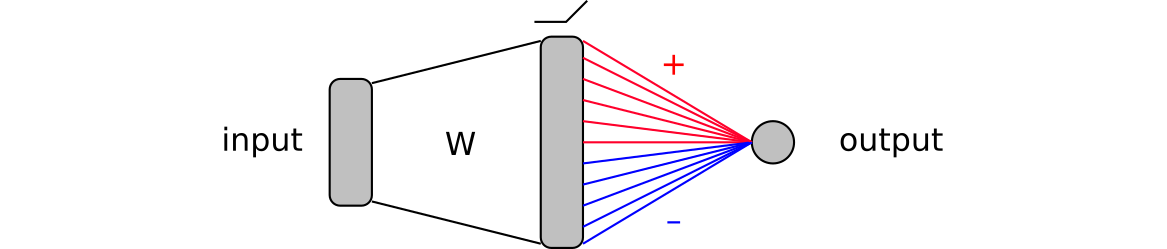
\includegraphics{neuralnet.png}
\caption{Diagram of the Neural Network Regressor used in this homework}
\end{figure}

The function \texttt{getarch} shown below generates an architecture
specific to the Boston housing dataset, with 13 input features,
\texttt{h} intermediate neurons, and one output. It takes as a parameter
the first layer type, which is usually \texttt{layers.Linear}. Later in
this homework, we will replace it by variants of \texttt{layers.Linear}
that incorporate weight norm penalties.

    \begin{Verbatim}[commandchars=\\\{\}]
{\color{incolor}In [{\color{incolor}2}]:} \PY{k+kn}{import} \PY{n+nn}{layers}
        
        \PY{k}{def} \PY{n+nf}{getarch}\PY{p}{(}\PY{n}{FirstLayerType}\PY{p}{)}\PY{p}{:}
            \PY{n}{h} \PY{o}{=} \PY{l+m+mi}{100}
            \PY{k}{return} \PY{n}{layers}\PY{o}{.}\PY{n}{Sequential}\PY{p}{(}\PY{p}{[}
                \PY{n}{FirstLayerType}\PY{p}{(}\PY{l+m+mi}{13}\PY{p}{,}\PY{n}{h}\PY{p}{,}\PY{n}{seed}\PY{o}{=}\PY{l+m+mi}{0}\PY{p}{)}\PY{p}{,}
                \PY{n}{layers}\PY{o}{.}\PY{n}{ReLU}\PY{p}{(}\PY{p}{)}\PY{p}{,}
                \PY{n}{layers}\PY{o}{.}\PY{n}{Pooling}\PY{p}{(}\PY{n}{h}\PY{p}{)}
            \PY{p}{]}\PY{p}{)}
\end{Verbatim}


    The class \texttt{NeuralNetworkRegressor} shown below takes a neural
network architecture, trains it on the data using gradient descent with
momentum, and predict new data points. Because the dataset is rather
small, we do not need to use stochastic gradient descent. We choose
instead the batch variant, where we follow the gradient of the true mean
square error.

    \begin{Verbatim}[commandchars=\\\{\}]
{\color{incolor}In [{\color{incolor}3}]:} \PY{k+kn}{import} \PY{n+nn}{sklearn}\PY{o}{,}\PY{n+nn}{sklearn}\PY{n+nn}{.}\PY{n+nn}{metrics}
        
        \PY{k}{class} \PY{n+nc}{NeuralNetworkRegressor}\PY{p}{:}
        
            \PY{k}{def} \PY{n+nf}{\PYZus{}\PYZus{}init\PYZus{}\PYZus{}}\PY{p}{(}\PY{n+nb+bp}{self}\PY{p}{,}\PY{n}{arch}\PY{p}{)}\PY{p}{:} \PY{n+nb+bp}{self}\PY{o}{.}\PY{n}{arch} \PY{o}{=} \PY{n}{arch}
        
            \PY{k}{def} \PY{n+nf}{fit}\PY{p}{(}\PY{n+nb+bp}{self}\PY{p}{,}\PY{n}{X}\PY{p}{,}\PY{n}{T}\PY{p}{,}\PY{n}{nbit}\PY{o}{=}\PY{l+m+mi}{10000}\PY{p}{)}\PY{p}{:}
        
                \PY{k}{for} \PY{n}{i} \PY{o+ow}{in} \PY{n+nb}{range}\PY{p}{(}\PY{n}{nbit}\PY{p}{)}\PY{p}{:}
                    \PY{n+nb+bp}{self}\PY{o}{.}\PY{n}{arch}\PY{o}{.}\PY{n}{backward}\PY{p}{(}\PY{l+m+mi}{2}\PY{o}{*}\PY{p}{(}\PY{n+nb+bp}{self}\PY{o}{.}\PY{n}{arch}\PY{o}{.}\PY{n}{forward}\PY{p}{(}\PY{n}{X}\PY{p}{)}\PY{o}{\PYZhy{}}\PY{n}{T}\PY{p}{)}\PY{p}{)}
                    \PY{k}{for} \PY{n}{l} \PY{o+ow}{in} \PY{n+nb+bp}{self}\PY{o}{.}\PY{n}{arch}\PY{o}{.}\PY{n}{layers}\PY{p}{:} \PY{n}{l}\PY{o}{.}\PY{n}{computepgrad}\PY{p}{(}\PY{p}{)}\PY{p}{;} \PY{n}{l}\PY{o}{.}\PY{n}{pgradstep}\PY{p}{(}\PY{l+m+mf}{0.01}\PY{p}{)}
                        
            \PY{k}{def} \PY{n+nf}{predict}\PY{p}{(}\PY{n+nb+bp}{self}\PY{p}{,}\PY{n}{X}\PY{p}{)}\PY{p}{:}
                \PY{k}{return} \PY{n+nb+bp}{self}\PY{o}{.}\PY{n}{arch}\PY{o}{.}\PY{n}{forward}\PY{p}{(}\PY{n}{X}\PY{p}{)}
        
            \PY{k}{def} \PY{n+nf}{score}\PY{p}{(}\PY{n+nb+bp}{self}\PY{p}{,}\PY{n}{X}\PY{p}{,}\PY{n}{T}\PY{p}{)}\PY{p}{:}
                \PY{k}{return} \PY{n}{sklearn}\PY{o}{.}\PY{n}{metrics}\PY{o}{.}\PY{n}{r2\PYZus{}score}\PY{p}{(}\PY{n}{T}\PY{p}{,}\PY{n+nb+bp}{self}\PY{o}{.}\PY{n}{predict}\PY{p}{(}\PY{n}{X}\PY{p}{)}\PY{p}{)}
\end{Verbatim}


    \subsubsection{Neural Network Performance vs.
Baselines}\label{neural-network-performance-vs.-baselines}

We compare the performance of the neural network on the Boston housing
data to two other regressors: a random forest and a support vector
regression model with RBF kernel. We use the scikit-learn implementation
of these models, with their default parameters.

    \begin{Verbatim}[commandchars=\\\{\}]
{\color{incolor}In [{\color{incolor}4}]:} \PY{k+kn}{import} \PY{n+nn}{sklearn}\PY{n+nn}{.}\PY{n+nn}{ensemble}\PY{o}{,}\PY{n+nn}{sklearn}\PY{n+nn}{.}\PY{n+nn}{svm}
        
        \PY{n}{rfr} \PY{o}{=} \PY{n}{sklearn}\PY{o}{.}\PY{n}{ensemble}\PY{o}{.}\PY{n}{RandomForestRegressor}\PY{p}{(}\PY{p}{)}
        \PY{n}{rfr}\PY{o}{.}\PY{n}{fit}\PY{p}{(}\PY{n}{Xtrain}\PY{p}{,}\PY{n}{Ttrain}\PY{p}{)}
        
        \PY{n}{svr} \PY{o}{=} \PY{n}{sklearn}\PY{o}{.}\PY{n}{svm}\PY{o}{.}\PY{n}{SVR}\PY{p}{(}\PY{p}{)}
        \PY{n}{svr}\PY{o}{.}\PY{n}{fit}\PY{p}{(}\PY{n}{Xtrain}\PY{p}{,}\PY{n}{Ttrain}\PY{p}{)}
        
        \PY{n}{nnr} \PY{o}{=} \PY{n}{NeuralNetworkRegressor}\PY{p}{(}\PY{n}{getarch}\PY{p}{(}\PY{n}{layers}\PY{o}{.}\PY{n}{Linear}\PY{p}{)}\PY{p}{)}
        \PY{n}{nnr}\PY{o}{.}\PY{n}{fit}\PY{p}{(}\PY{n}{Xtrain}\PY{p}{,}\PY{n}{Ttrain}\PY{p}{)}
\end{Verbatim}


    \begin{Verbatim}[commandchars=\\\{\}]
{\color{incolor}In [{\color{incolor}5}]:} \PY{k}{def} \PY{n+nf}{pretty}\PY{p}{(}\PY{n}{name}\PY{p}{,}\PY{n}{model}\PY{p}{)}\PY{p}{:}
            \PY{k}{return} \PY{l+s+s1}{\PYZsq{}}\PY{l+s+s1}{\PYZgt{} }\PY{l+s+si}{\PYZpc{}10s}\PY{l+s+s1}{ | R2train: }\PY{l+s+si}{\PYZpc{}6.3f}\PY{l+s+s1}{ | R2test: }\PY{l+s+si}{\PYZpc{}6.3f}\PY{l+s+s1}{\PYZsq{}}\PY{o}{\PYZpc{}}\PY{p}{(}\PY{n}{name}\PY{p}{,}\PY{n}{model}\PY{o}{.}\PY{n}{score}\PY{p}{(}\PY{n}{Xtrain}\PY{p}{,}\PY{n}{Ttrain}\PY{p}{)}\PY{p}{,}\PY{n}{model}\PY{o}{.}\PY{n}{score}\PY{p}{(}\PY{n}{Xtest}\PY{p}{,}\PY{n}{Ttest}\PY{p}{)}\PY{p}{)}
        
        \PY{n+nb}{print}\PY{p}{(}\PY{n}{pretty}\PY{p}{(}\PY{l+s+s1}{\PYZsq{}}\PY{l+s+s1}{RForest}\PY{l+s+s1}{\PYZsq{}}\PY{p}{,}\PY{n}{rfr}\PY{p}{)}\PY{p}{)}
        \PY{n+nb}{print}\PY{p}{(}\PY{n}{pretty}\PY{p}{(}\PY{l+s+s1}{\PYZsq{}}\PY{l+s+s1}{SVR}\PY{l+s+s1}{\PYZsq{}}\PY{p}{,}\PY{n}{svr}\PY{p}{)}\PY{p}{)}
        \PY{n+nb}{print}\PY{p}{(}\PY{n}{pretty}\PY{p}{(}\PY{l+s+s1}{\PYZsq{}}\PY{l+s+s1}{NNreg}\PY{l+s+s1}{\PYZsq{}}\PY{p}{,}\PY{n}{nnr}\PY{p}{)}\PY{p}{)}
\end{Verbatim}


    \begin{Verbatim}[commandchars=\\\{\}]
>    RForest | R2train:  0.970 | R2test:  0.845
>        SVR | R2train:  0.913 | R2test:  0.758
>      NNreg | R2train:  0.996 | R2test:  0.845

    \end{Verbatim}

    The neural networks performs on par with the other regression models
although it has in principle the added ability to learn its own internal
features. We would therefore expect a well-trained neural network to
perform better.

\subsection{Gradient, and Parameter Norms (20
P)}\label{gradient-and-parameter-norms-20-p}

As a first step towards improving the neural network model, we will
measure proxy quantities, that will then be used to regularize the
model. We consider the following three quantities:

\begin{itemize}
\tightlist
\item
  \(\|W\|_\text{Frob} = \sqrt{\sum_{i=1}^d \sum_{j=1}^h w_{ij}^2}\)
\item
  \(\|W\|_\text{Mix} = h^{-0.5} \sqrt{\sum_{i=1}^d \big(\sum_{j=1}^h | w_{ij}|\big)^2}\)
\item
  \(\text{Grad} = \textstyle \frac1N \sum_{n=1}^N\|\nabla_{\boldsymbol{x}}f (\boldsymbol{x_n})\|\)
\end{itemize}

where \(d\) is the number of input features, \(h\) is the number of
neurons in the hidden layer, and \(W\) is the matrix of weights in the
first layer. In order for the model to generalize well, the last
quantity (\(\text{Grad}\)) should be prevented from becoming too large.
Because the latter depends on the data distribution, we rely instead on
the inequality
\(\text{Grad} \leq \|W\|_\text{Mix} \leq \|W\|_\text{Frob}\), that we
can prove for this model, and will try to control the weight norms
instead.

\paragraph{Tasks:}\label{tasks}

\begin{itemize}
\tightlist
\item
  Implement the function \texttt{WMix(nn)} that receives the neural
  network as input and returns \(\|W\|_\text{Mix}\).
\item
  Implement the function \texttt{Grad(nn,X)} that receives the neural
  network and some dataset as input, and computes the averaged gradient
  norm (\(\text{Grad}\)).
\end{itemize}

    \begin{Verbatim}[commandchars=\\\{\}]
{\color{incolor}In [{\color{incolor}6}]:} \PY{k}{def} \PY{n+nf}{WFrob}\PY{p}{(}\PY{n}{nn}\PY{p}{)}\PY{p}{:}
            \PY{n}{W} \PY{o}{=} \PY{n}{nn}\PY{o}{.}\PY{n}{arch}\PY{o}{.}\PY{n}{layers}\PY{p}{[}\PY{l+m+mi}{0}\PY{p}{]}\PY{o}{.}\PY{n}{W}
            \PY{k}{return} \PY{p}{(}\PY{n}{W}\PY{o}{*}\PY{o}{*}\PY{l+m+mi}{2}\PY{p}{)}\PY{o}{.}\PY{n}{sum}\PY{p}{(}\PY{p}{)}\PY{o}{*}\PY{o}{*}\PY{o}{.}\PY{l+m+mi}{5}
        
        \PY{k}{def} \PY{n+nf}{WMix}\PY{p}{(}\PY{n}{nn}\PY{p}{)}\PY{p}{:}
            \PY{n}{W} \PY{o}{=} \PY{n}{nn}\PY{o}{.}\PY{n}{arch}\PY{o}{.}\PY{n}{layers}\PY{p}{[}\PY{l+m+mi}{0}\PY{p}{]}\PY{o}{.}\PY{n}{W}
            \PY{k}{return} \PY{p}{(}\PY{l+m+mi}{1} \PY{o}{/} \PY{n}{W}\PY{o}{.}\PY{n}{shape}\PY{p}{[}\PY{l+m+mi}{1}\PY{p}{]} \PY{o}{*} \PY{p}{(}\PY{n+nb}{abs}\PY{p}{(}\PY{n}{W}\PY{p}{)}\PY{o}{.}\PY{n}{sum}\PY{p}{(}\PY{n}{axis} \PY{o}{=} \PY{l+m+mi}{1}\PY{p}{)} \PY{o}{*}\PY{o}{*} \PY{l+m+mi}{2}\PY{p}{)}\PY{o}{.}\PY{n}{sum}\PY{p}{(}\PY{p}{)}\PY{p}{)}\PY{o}{*}\PY{o}{*}\PY{l+m+mf}{0.5}
        \PY{k+kn}{import} \PY{n+nn}{numpy} \PY{k}{as} \PY{n+nn}{np}
        
        \PY{k}{def} \PY{n+nf}{Grad}\PY{p}{(}\PY{n}{nn}\PY{p}{,}\PY{n}{X}\PY{p}{)}\PY{p}{:}
            \PY{n}{W} \PY{o}{=} \PY{n}{nn}\PY{o}{.}\PY{n}{arch}\PY{o}{.}\PY{n}{layers}\PY{p}{[}\PY{l+m+mi}{0}\PY{p}{]}\PY{o}{.}\PY{n}{W}
            \PY{n}{B} \PY{o}{=} \PY{n}{nn}\PY{o}{.}\PY{n}{arch}\PY{o}{.}\PY{n}{layers}\PY{p}{[}\PY{l+m+mi}{0}\PY{p}{]}\PY{o}{.}\PY{n}{B}
            \PY{k}{def} \PY{n+nf}{grad1}\PY{p}{(}\PY{n}{X}\PY{p}{,}\PY{n}{W}\PY{p}{,}\PY{n}{B}\PY{p}{)}\PY{p}{:}
                \PY{n}{s} \PY{o}{=} \PY{n}{np}\PY{o}{.}\PY{n}{zeros}\PY{p}{(}\PY{n}{W}\PY{o}{.}\PY{n}{shape}\PY{p}{[}\PY{l+m+mi}{0}\PY{p}{]}\PY{p}{)}
                \PY{k}{for} \PY{n}{j} \PY{o+ow}{in} \PY{n+nb}{range}\PY{p}{(}\PY{n}{W}\PY{o}{.}\PY{n}{shape}\PY{p}{[}\PY{l+m+mi}{1}\PY{p}{]}\PY{p}{)}\PY{p}{:}
                    \PY{n}{I} \PY{o}{=} \PY{n}{X}\PY{o}{.}\PY{n}{dot}\PY{p}{(}\PY{n}{W}\PY{p}{[}\PY{p}{:}\PY{p}{,}\PY{n}{j}\PY{p}{]}\PY{p}{)} \PY{o}{+} \PY{n}{B}\PY{p}{[}\PY{n}{j}\PY{p}{]} \PY{o}{\PYZgt{}} \PY{l+m+mi}{0}
                    \PY{n}{s} \PY{o}{+}\PY{o}{=} \PY{n}{W}\PY{p}{[}\PY{p}{:}\PY{p}{,}\PY{n}{j}\PY{p}{]} \PY{o}{*} \PY{n}{I}
                \PY{k}{return} \PY{p}{(}\PY{n}{s}\PY{o}{*}\PY{o}{*}\PY{l+m+mi}{2}\PY{p}{)}\PY{o}{.}\PY{n}{sum}\PY{p}{(}\PY{p}{)}\PY{o}{*}\PY{o}{*}\PY{l+m+mf}{0.5}
            \PY{n}{ret} \PY{o}{=} \PY{n}{np}\PY{o}{.}\PY{n}{mean}\PY{p}{(}\PY{p}{[}\PY{n}{grad1}\PY{p}{(}\PY{n}{x}\PY{p}{,}\PY{n}{W}\PY{p}{,}\PY{n}{B}\PY{p}{)} \PY{k}{for} \PY{n}{x} \PY{o+ow}{in} \PY{n}{X}\PY{p}{]}\PY{p}{)}
            \PY{k}{return} \PY{n}{ret}
\end{Verbatim}


    The following experiment computes these three quantities before and
after training the model.

    \begin{Verbatim}[commandchars=\\\{\}]
{\color{incolor}In [{\color{incolor}7}]:} \PY{k}{global} \PY{n}{count} 
        \PY{n}{count} \PY{o}{=} \PY{l+m+mi}{0}
        \PY{k}{def} \PY{n+nf}{fullpretty}\PY{p}{(}\PY{n}{name}\PY{p}{,}\PY{n}{nn}\PY{p}{)}\PY{p}{:}
            \PY{k}{return} \PY{n}{pretty}\PY{p}{(}\PY{n}{name}\PY{p}{,}\PY{n}{nn}\PY{p}{)} \PY{o}{+} \PY{l+s+s1}{\PYZsq{}}\PY{l+s+s1}{ | WFrob: }\PY{l+s+si}{\PYZpc{}7.3f}\PY{l+s+s1}{ | WMix: }\PY{l+s+si}{\PYZpc{}7.3f}\PY{l+s+s1}{ | Grad: }\PY{l+s+si}{\PYZpc{}7.3f}\PY{l+s+s1}{\PYZsq{}}\PY{o}{\PYZpc{}}\PY{p}{(}\PY{n}{WFrob}\PY{p}{(}\PY{n}{nn}\PY{p}{)}\PY{p}{,}\PY{n}{WMix}\PY{p}{(}\PY{n}{nn}\PY{p}{)}\PY{p}{,}\PY{n}{Grad}\PY{p}{(}\PY{n}{nn}\PY{p}{,}\PY{n}{Xtest}\PY{p}{)}\PY{p}{)}
        
        \PY{n}{nnr} \PY{o}{=} \PY{n}{NeuralNetworkRegressor}\PY{p}{(}\PY{n}{getarch}\PY{p}{(}\PY{n}{layers}\PY{o}{.}\PY{n}{Linear}\PY{p}{)}\PY{p}{)}
        \PY{n+nb}{print}\PY{p}{(}\PY{n}{fullpretty}\PY{p}{(}\PY{l+s+s1}{\PYZsq{}}\PY{l+s+s1}{Before}\PY{l+s+s1}{\PYZsq{}}\PY{p}{,}\PY{n}{nnr}\PY{p}{)}\PY{p}{)}
        \PY{n}{nnr}\PY{o}{.}\PY{n}{fit}\PY{p}{(}\PY{n}{Xtrain}\PY{p}{,}\PY{n}{Ttrain}\PY{p}{)}
        \PY{n+nb}{print}\PY{p}{(}\PY{n}{fullpretty}\PY{p}{(}\PY{l+s+s1}{\PYZsq{}}\PY{l+s+s1}{After}\PY{l+s+s1}{\PYZsq{}}\PY{p}{,}\PY{n}{nnr}\PY{p}{)}\PY{p}{)}
\end{Verbatim}


    \begin{Verbatim}[commandchars=\\\{\}]
>     Before | R2train: -0.043 | R2test: -0.006 | WFrob:   9.834 | WMix:   7.845 | Grad:  13.562
>      After | R2train:  0.996 | R2test:  0.845 | WFrob:  18.752 | WMix:  15.018 | Grad:  26.402

    \end{Verbatim}

    We observe that the inequality
\(\text{Grad} \leq \|W\|_\text{Mix} < \|W\|_\text{Frob}\) also holds
empirically. We also observe that these quantities tend to increase as
training proceeds. This is a typical behavior, as the network starts
rather simple and becomes complex as more and more variations in the
training data are being captured.

    \subsection{Frobenius-Norm Penalty (10
P)}\label{frobenius-norm-penalty-10-p}

The first penalty we experiment with is the squared Frobenius norm. We
consider the new objective
\(J^\text{Frob}(\theta) = \text{MSE}(\theta) + \lambda \cdot \|W\|_\text{Frob}^2\),
where the first term is the original mean square error objective and
where the second term is the added penalty. We hardcode the penalty
coeffecient to \(\lambda = 10^{-3}\). In principle, for maximum
performance and fair comparison between the methods, several of them
should be tried (also for other models), and selected based on some
validation set. Here, for simplicity, we omit this step.

\paragraph{Tasks:}\label{tasks}

\begin{itemize}
\tightlist
\item
  Create a new layer, that replaces the original \texttt{layers.Linear}
  layer and incorporates the proposed penalty. \emph{(Hint: This can be
  achieved by extending layers.Linear, and rewriting its method
  \texttt{computepgrad}.)}
\end{itemize}

    \begin{Verbatim}[commandchars=\\\{\}]
{\color{incolor}In [{\color{incolor}8}]:} \PY{c+c1}{\PYZsh{} \PYZhy{}\PYZhy{}\PYZhy{}\PYZhy{}\PYZhy{}\PYZhy{}\PYZhy{}\PYZhy{}\PYZhy{}\PYZhy{}\PYZhy{}\PYZhy{}\PYZhy{}\PYZhy{}\PYZhy{}\PYZhy{}\PYZhy{}\PYZhy{}\PYZhy{}\PYZhy{}\PYZhy{}\PYZhy{}\PYZhy{}\PYZhy{}\PYZhy{}\PYZhy{}\PYZhy{}\PYZhy{}\PYZhy{}\PYZhy{}\PYZhy{}\PYZhy{}\PYZhy{}\PYZhy{}\PYZhy{}\PYZhy{}\PYZhy{}\PYZhy{}\PYZhy{}\PYZhy{}\PYZhy{}\PYZhy{}}
        \PY{c+c1}{\PYZsh{} TODO: Replace by your code}
        \PY{c+c1}{\PYZsh{} \PYZhy{}\PYZhy{}\PYZhy{}\PYZhy{}\PYZhy{}\PYZhy{}\PYZhy{}\PYZhy{}\PYZhy{}\PYZhy{}\PYZhy{}\PYZhy{}\PYZhy{}\PYZhy{}\PYZhy{}\PYZhy{}\PYZhy{}\PYZhy{}\PYZhy{}\PYZhy{}\PYZhy{}\PYZhy{}\PYZhy{}\PYZhy{}\PYZhy{}\PYZhy{}\PYZhy{}\PYZhy{}\PYZhy{}\PYZhy{}\PYZhy{}\PYZhy{}\PYZhy{}\PYZhy{}\PYZhy{}\PYZhy{}\PYZhy{}\PYZhy{}\PYZhy{}\PYZhy{}\PYZhy{}\PYZhy{}}
        \PY{c+c1}{\PYZsh{} import solution}
        \PY{c+c1}{\PYZsh{} LinearFrob = solution.LinearFrob}
        \PY{k+kn}{import} \PY{n+nn}{copy}
        \PY{n}{LinearFrob} \PY{o}{=} \PY{n}{copy}\PY{o}{.}\PY{n}{deepcopy}\PY{p}{(}\PY{n}{layers}\PY{o}{.}\PY{n}{Linear}\PY{p}{)}
        \PY{k}{def} \PY{n+nf}{computepgradFrob} \PY{p}{(}\PY{n+nb+bp}{self}\PY{p}{,}\PY{n}{lam} \PY{o}{=} \PY{l+m+mi}{1}\PY{o}{/}\PY{l+m+mi}{10}\PY{o}{*}\PY{o}{*}\PY{l+m+mi}{3}\PY{p}{)}\PY{p}{:}
            \PY{n+nb+bp}{self}\PY{o}{.}\PY{n}{DW} \PY{o}{=} \PY{n}{np}\PY{o}{.}\PY{n}{dot}\PY{p}{(}\PY{n+nb+bp}{self}\PY{o}{.}\PY{n}{A}\PY{o}{.}\PY{n}{T}\PY{p}{,}\PY{n+nb+bp}{self}\PY{o}{.}\PY{n}{DZ}\PY{p}{)}\PY{o}{/}\PY{n+nb}{len}\PY{p}{(}\PY{n+nb+bp}{self}\PY{o}{.}\PY{n}{A}\PY{p}{)} \PY{o}{+} \PY{n}{lam} \PY{o}{*}\PY{l+m+mi}{2} \PY{o}{*} \PY{n+nb+bp}{self}\PY{o}{.}\PY{n}{W}
            \PY{n+nb+bp}{self}\PY{o}{.}\PY{n}{DB} \PY{o}{=} \PY{n+nb+bp}{self}\PY{o}{.}\PY{n}{DZ}\PY{o}{.}\PY{n}{mean}\PY{p}{(}\PY{n}{axis}\PY{o}{=}\PY{l+m+mi}{0}\PY{p}{)}
        \PY{n}{LinearFrob}\PY{o}{.}\PY{n}{computepgrad} \PY{o}{=} \PY{n}{computepgradFrob}
        
        \PY{c+c1}{\PYZsh{} \PYZhy{}\PYZhy{}\PYZhy{}\PYZhy{}\PYZhy{}\PYZhy{}\PYZhy{}\PYZhy{}\PYZhy{}\PYZhy{}\PYZhy{}\PYZhy{}\PYZhy{}\PYZhy{}\PYZhy{}\PYZhy{}\PYZhy{}\PYZhy{}\PYZhy{}\PYZhy{}\PYZhy{}\PYZhy{}\PYZhy{}\PYZhy{}\PYZhy{}\PYZhy{}\PYZhy{}\PYZhy{}\PYZhy{}\PYZhy{}\PYZhy{}\PYZhy{}\PYZhy{}\PYZhy{}\PYZhy{}\PYZhy{}\PYZhy{}\PYZhy{}\PYZhy{}\PYZhy{}\PYZhy{}\PYZhy{}}
\end{Verbatim}


    The code below trains a neural network with the new first layer, and
compares the performance with the previous models.

    \begin{Verbatim}[commandchars=\\\{\}]
{\color{incolor}In [{\color{incolor}9}]:} \PY{n}{nnfrob} \PY{o}{=} \PY{n}{NeuralNetworkRegressor}\PY{p}{(}\PY{n}{getarch}\PY{p}{(}\PY{n}{LinearFrob}\PY{p}{)}\PY{p}{)}
        \PY{n}{nnfrob}\PY{o}{.}\PY{n}{fit}\PY{p}{(}\PY{n}{Xtrain}\PY{p}{,}\PY{n}{Ttrain}\PY{p}{)}
\end{Verbatim}


    \begin{Verbatim}[commandchars=\\\{\}]
{\color{incolor}In [{\color{incolor}10}]:} \PY{n+nb}{print}\PY{p}{(}\PY{n}{pretty}\PY{p}{(}\PY{l+s+s1}{\PYZsq{}}\PY{l+s+s1}{RForest}\PY{l+s+s1}{\PYZsq{}}\PY{p}{,}\PY{n}{rfr}\PY{p}{)}\PY{p}{)}
         \PY{n+nb}{print}\PY{p}{(}\PY{n}{pretty}\PY{p}{(}\PY{l+s+s1}{\PYZsq{}}\PY{l+s+s1}{SVR}\PY{l+s+s1}{\PYZsq{}}\PY{p}{,}\PY{n}{svr}\PY{p}{)}\PY{p}{)}
         \PY{n+nb}{print}\PY{p}{(}\PY{n}{fullpretty}\PY{p}{(}\PY{l+s+s1}{\PYZsq{}}\PY{l+s+s1}{NN}\PY{l+s+s1}{\PYZsq{}}\PY{p}{,}\PY{n}{nnr}\PY{p}{)}\PY{p}{)}
         \PY{n+nb}{print}\PY{p}{(}\PY{n}{fullpretty}\PY{p}{(}\PY{l+s+s1}{\PYZsq{}}\PY{l+s+s1}{NN+Frob}\PY{l+s+s1}{\PYZsq{}}\PY{p}{,}\PY{n}{nnfrob}\PY{p}{)}\PY{p}{)}
\end{Verbatim}


    \begin{Verbatim}[commandchars=\\\{\}]
>    RForest | R2train:  0.970 | R2test:  0.845
>        SVR | R2train:  0.913 | R2test:  0.758
>         NN | R2train:  0.996 | R2test:  0.845 | WFrob:  18.752 | WMix:  15.018 | Grad:  26.402
>    NN+Frob | R2train:  0.967 | R2test:  0.833 | WFrob:   5.119 | WMix:   4.139 | Grad:   7.263

    \end{Verbatim}

    As we can see, the penalty has the effect of strongly reducing the
Frobenius norm of the weight matrix. However, the test accuracy is not
improved.

    \subsection{Mixed-Norm Penalty (10 P)}\label{mixed-norm-penalty-10-p}

A downside of the Frobenius norm is that it is not a very tight upper
bound of the gradient, that is, penalizing it is does not penalize
specifically high gradient. Instead, other useful properties of the
model could be negatively affected by it. In the following, we
experiment with the mixed-norm regularizer, which is a tighter bound of
the gradient.

The objective function is now given by
\(\textstyle J^{\text{Mix}}(\theta) = \text{MSE}(\theta) + \lambda \cdot \|W\|_\text{Mix}^2\)
, where the first and second terms are again the original objective and
the penalty term. As for the previous exercise, we hardcode the latter
coefficient to \(10^{-3}\).

\paragraph{Tasks:}\label{tasks}

\begin{itemize}
\tightlist
\item
  Using the same technique as before, create a new layer that
  incorporates the Mixed norm penalty.
\end{itemize}

The differential of the Mix norm for element \(W_{l,k}\) is $
\frac{\partial\|W\|_\text{Mix}^2}{\partial W_{l,k}} =
2h^{-1}\sum_{i=1}^{h}W_{l,j}\text{sign}(W_{l,k})
=
2h^{-1}W_{l,:}1\text{sign}(W_{l,k})
$ thus
\(\frac{\partial\|W\|_\text{Mix}^2}{\partial W}  = 2h^{-1}\tilde{W}_{(1)} 1_h^T \odot\text{sign}(W)\)
with \(\tilde{W}_{(1)} := (\|W_{1,:}\|_1, ..., \|W_{d,:}\|_1)^T\).
Reminder: \(\odot\) represents the operator for the elemente-wise matrix
multiplication.

    \begin{Verbatim}[commandchars=\\\{\}]
{\color{incolor}In [{\color{incolor}11}]:} \PY{n}{LinearMix} \PY{o}{=} \PY{n}{copy}\PY{o}{.}\PY{n}{deepcopy}\PY{p}{(}\PY{n}{layers}\PY{o}{.}\PY{n}{Linear}\PY{p}{)}
         \PY{k}{def} \PY{n+nf}{computepgradMix} \PY{p}{(}\PY{n+nb+bp}{self}\PY{p}{,}\PY{n}{lam} \PY{o}{=} \PY{l+m+mi}{1}\PY{o}{/}\PY{l+m+mi}{10}\PY{o}{*}\PY{o}{*}\PY{l+m+mi}{3}\PY{p}{)}\PY{p}{:}
             \PY{n}{\PYZus{}W2} \PY{o}{=} \PY{n}{np}\PY{o}{.}\PY{n}{outer}\PY{p}{(}\PY{n+nb}{abs}\PY{p}{(}\PY{n+nb+bp}{self}\PY{o}{.}\PY{n}{W}\PY{p}{)}\PY{o}{.}\PY{n}{sum}\PY{p}{(}\PY{n}{axis}\PY{o}{=} \PY{l+m+mi}{1}\PY{p}{)}\PY{p}{,}\PY{n}{np}\PY{o}{.}\PY{n}{ones}\PY{p}{(}\PY{n+nb+bp}{self}\PY{o}{.}\PY{n}{W}\PY{o}{.}\PY{n}{shape}\PY{p}{[}\PY{l+m+mi}{1}\PY{p}{]}\PY{p}{)}\PY{p}{)}
             \PY{n+nb+bp}{self}\PY{o}{.}\PY{n}{DW} \PY{o}{=} \PY{n}{np}\PY{o}{.}\PY{n}{dot}\PY{p}{(}\PY{n+nb+bp}{self}\PY{o}{.}\PY{n}{A}\PY{o}{.}\PY{n}{T}\PY{p}{,}\PY{n+nb+bp}{self}\PY{o}{.}\PY{n}{DZ}\PY{p}{)}\PY{o}{/}\PY{n+nb}{len}\PY{p}{(}\PY{n+nb+bp}{self}\PY{o}{.}\PY{n}{A}\PY{p}{)} 
             \PY{n+nb+bp}{self}\PY{o}{.}\PY{n}{DW}\PY{o}{+}\PY{o}{=} \PY{n}{lam} \PY{o}{*} \PY{l+m+mi}{2} \PY{o}{/} \PY{n+nb+bp}{self}\PY{o}{.}\PY{n}{W}\PY{o}{.}\PY{n}{shape}\PY{p}{[}\PY{l+m+mi}{1}\PY{p}{]} \PY{o}{*} \PY{n}{np}\PY{o}{.}\PY{n}{multiply}\PY{p}{(}\PY{n}{\PYZus{}W2}\PY{p}{,}\PY{n}{np}\PY{o}{.}\PY{n}{sign}\PY{p}{(}\PY{n+nb+bp}{self}\PY{o}{.}\PY{n}{W}\PY{p}{)}\PY{p}{)}
             \PY{n+nb+bp}{self}\PY{o}{.}\PY{n}{DB} \PY{o}{=} \PY{n+nb+bp}{self}\PY{o}{.}\PY{n}{DZ}\PY{o}{.}\PY{n}{mean}\PY{p}{(}\PY{n}{axis}\PY{o}{=}\PY{l+m+mi}{0}\PY{p}{)}
         \PY{n}{LinearMix}\PY{o}{.}\PY{n}{computepgrad} \PY{o}{=} \PY{n}{computepgradMix}
\end{Verbatim}


    The code below trains a neural network with the new penalty, and
compares the performance with the previous models.

    \begin{Verbatim}[commandchars=\\\{\}]
{\color{incolor}In [{\color{incolor}12}]:} \PY{n}{nnmix} \PY{o}{=} \PY{n}{NeuralNetworkRegressor}\PY{p}{(}\PY{n}{getarch}\PY{p}{(}\PY{n}{LinearMix}\PY{p}{)}\PY{p}{)}
         \PY{n}{nnmix}\PY{o}{.}\PY{n}{fit}\PY{p}{(}\PY{n}{Xtrain}\PY{p}{,}\PY{n}{Ttrain}\PY{p}{)}
\end{Verbatim}


    \begin{Verbatim}[commandchars=\\\{\}]
{\color{incolor}In [{\color{incolor}13}]:} \PY{n+nb}{print}\PY{p}{(}\PY{n}{pretty}\PY{p}{(}\PY{l+s+s1}{\PYZsq{}}\PY{l+s+s1}{RForest}\PY{l+s+s1}{\PYZsq{}}\PY{p}{,}\PY{n}{rfr}\PY{p}{)}\PY{p}{)}
         \PY{n+nb}{print}\PY{p}{(}\PY{n}{pretty}\PY{p}{(}\PY{l+s+s1}{\PYZsq{}}\PY{l+s+s1}{SVR}\PY{l+s+s1}{\PYZsq{}}\PY{p}{,}\PY{n}{svr}\PY{p}{)}\PY{p}{)}
         \PY{n+nb}{print}\PY{p}{(}\PY{n}{fullpretty}\PY{p}{(}\PY{l+s+s1}{\PYZsq{}}\PY{l+s+s1}{NN}\PY{l+s+s1}{\PYZsq{}}\PY{p}{,}\PY{n}{nnr}\PY{p}{)}\PY{p}{)}
         \PY{n+nb}{print}\PY{p}{(}\PY{n}{fullpretty}\PY{p}{(}\PY{l+s+s1}{\PYZsq{}}\PY{l+s+s1}{NN+Frob}\PY{l+s+s1}{\PYZsq{}}\PY{p}{,}\PY{n}{nnfrob}\PY{p}{)}\PY{p}{)}
         \PY{n+nb}{print}\PY{p}{(}\PY{n}{fullpretty}\PY{p}{(}\PY{l+s+s1}{\PYZsq{}}\PY{l+s+s1}{NN+Mix}\PY{l+s+s1}{\PYZsq{}}\PY{p}{,}\PY{n}{nnmix}\PY{p}{)}\PY{p}{)}
\end{Verbatim}


    \begin{Verbatim}[commandchars=\\\{\}]
>    RForest | R2train:  0.970 | R2test:  0.845
>        SVR | R2train:  0.913 | R2test:  0.758
>         NN | R2train:  0.996 | R2test:  0.845 | WFrob:  18.752 | WMix:  15.018 | Grad:  26.402
>    NN+Frob | R2train:  0.967 | R2test:  0.833 | WFrob:   5.119 | WMix:   4.139 | Grad:   7.263
>     NN+Mix | R2train:  0.978 | R2test:  0.856 | WFrob:   8.188 | WMix:   4.214 | Grad:   8.821

    \end{Verbatim}

    It is interesting to observe that this mixed norm penalty more
selectively reduced the mixed norm and the gradient, and has let the
Frobenius norm take higher values. The mixed-norm model is also the one
that produces the highest test set accuracy.


    % Add a bibliography block to the postdoc
    
    
    
    \end{document}
